%!TEX root = ../CombinatoricsNotes.tex

\section{Convexity}
We will consider finite collections of points in Euclidean space, $\R^d$. Let's recall some definitions.
\begin{itemize}[]
\item[Linear space:] $L\subset \R^d$ is a \defn{linear space}[linear!space] if it is closed under addition and multiplication by scalars.
\item[Linear dependence:] We say $v_1,v_2,\dotsc,v_n$ are \defn{linearly dependent}[linear!dependence] if there exist $\alpha_1,\alpha_2,\dotsc,\alpha_n\in \R$ not all zero such that
\[
\alpha_1 v_1 + \alpha_2v_2 + \dotsc + \alpha_n v_n = 0.
\]
\item[Linear hull:] The \defn{linear hull}[linear!hull] $\braket{S}$ of $S\subset \R^d$ is the smallest linear subspace containing $S$, i.e. $\braket{S}=\bigcap_{L\supset S} L$ where the intersection is taken over linear subspaces $L$. Equivalently,
\begin{align*}	
\braket{S} = \{ \alpha_1 v_1 + \alpha_2 v_2 + \dotsc + \alpha_n v_n: \forall n,\, v_1,\dotsc,v_n\in S,\, \alpha_1,\dotsc,\alpha_n\in \R \}.
\end{align*}
Note that we may take $n = d$.
% , because any $d+1$ vectors in $S\subset \R^d$ will be linearly dependent.}

\item[Affine subspace:] An \defn{affine subspace}[affine!subspace] is a subset of $\R^d$ of the form $v+ L$ where $L$ is a linear subspace and $v\in \R^d$.

\item[Affine hull:] The \defn{affine hull}[affine!hull] $\aff(S)$ of $S\subset \R^d$ is the intersection of all affine subspaces containing $S$. Equivalently,
\[
\aff(S) = \{\alpha_1 v_1 + \alpha_2 v_2 + \dotsb + \alpha_n v_n : \sum_i \alpha_i= 1,\, v_1,\dotsc,v_n\in S\}.
\]
Note: if $w\in v+L$, then $w-v\in L$, so $w+L = v+L$. 

\item[Affine dependence:]A set of vectors $\{v_1,\dotsc,v_n\}$ are \defn{affinely dependent}[affine!dependence] if 
\[
\alpha_1 v_1 + \dotsb + \alpha_n v_n = 0
\]
for some $\sum_{i=1}^n\alpha_i=0$ with some $\alpha_i \neq 0$. This is equivalent to one of the vectors belongs to the affine hull of the other vectors.
\begin{remark}
The maximum number of affinely independent vectors in $\R^d$ is $d+1$. Why? Any $d+2$ vectors in $\R^d$ are affinely dependent. Suppose we have $v_1,\dotsc,v_{d+2}$. Then WLOG $v_1,\dotsc,v_d$ form a basis of $\R^d$. Then $\alpha_1 v_1 + \dotsb + \alpha_d v_d = v_{d+1}$ for some choice of $\alpha_i$'s. Likewise, $\beta_1 v_1  +\dotsb + \beta_d v_d = v_{d+2}$. Let $\alpha = \sum_i \alpha_i$ and $\beta = \sum_i \beta_i$. So
\begin{align*}	
\alpha_1 v_1 + \dotsb + \alpha_d v_d - v_{d+1} &= 0\\
\beta_1 v_1 + \dotsb + \beta_d v_d - v_{d+2} &= 0.
\end{align*}If $\alpha=1$ or $\beta=1$, then we are done. Otherwise,
\begin{align*}	
(\beta-1)(\alpha_1 v_1 + \dotsb + \alpha_d v_d - v_{d+1}) - (\alpha-1)(\beta_1 v_1 + \dotsb + \beta_d v_d - v_{d+2} ) &= 0
\end{align*}
which demonstrates affine dependence, as the sum of coefficients is $(\beta-1)(\alpha-1) - (\alpha-1)(\beta-1)=0$.
\end{remark}


\item[Convex:] A set $C\subset \R^d$ is \defn{convex} if for any two points $v_1,v_2\in C$, the interval joining these two points lies in $C$. That is, if $v_1,v_2\in C$, then $\{\alpha v_1 + (1- \alpha)v_2: 0\leq \alpha \leq 1\} \subset C$.
\item[Convex hull:]  For $X\subset \R^d$, the \defn{convex hull}[convex!hull] $\conv(X)$ is the intersection of all convex sets containing $X$. Then
\[
\conv(X) = \{\alpha_1 v_1 + \dotsc + \alpha_n v_n:n\in \N,\, v_1,\dotsc,v_n\in X, \sum_i \alpha_i =1, \alpha_i\geq 0 \}
\]
Note that $\alpha_1 v_1 + \dotsc + \alpha_n v_n$ where $\alpha_i\geq 0$ and $\sum_i \alpha_i=1$ is called a \defn{convex combination}[convex!combination] of $v_1,\dotsc,v_n$.

To prove this formula,  we note by induction on $n$ we see that any convex combination of $n$ vectors in $X$ is in $\conv(X)$: wlog $\alpha_n\neq 0$, $\alpha_n\neq 1$. Then 
\[
\alpha_1 v_1 + \dotsc + \alpha_n v_n = (1- \alpha_n) \underbrace{\left[ \frac{\alpha_1}{1- \alpha_n}v_1 + \dotsc + \frac{\alpha_{n-1}}{1 - \alpha_n} v_{n-1} \right]}_{\in \conv(X)} + \alpha_n \underbrace{ v_n.}_{\in \conv(X)}
\]
So this set of convex combinations is a subset of $\conv(X)$. But since the set of convex combinations is itself convex, as it is easy to check, we have equality.

\item[Convex dependence:]We say $X\subset \R^d$  is \defn{convex dependent}[convex!dependence] if for some $x\in X$ we have $x\in \conv(X\setminus \{x\})$. \marginnote{That is, one vector in $X$ is a convex combination of some of the others.}

We say $X$ is \defn{convex independent}[convex!independence] if it is not convex dependent.

\begin{remark}
No point on the boundary of a circle is a convex combination of the other points, so there is no bound on the size of convex independent sets.
\end{remark}

\end{itemize}


\begin{theorem}[\cite{Radon1921}] 
Let $A\subset \R^d$ be finite, with $|A| \geq d+2$. Then there exist disjoint $A_1,A_2\subset A$ such that $\conv(A_1)\cap \conv(A_2)\neq 0$.

\end{theorem}
\begin{remark}
Let's first consider the case $d=2$, $|A| =4$. If three points do not fall on a line (a degenerate case), then there are two cases: 
\begin{figure}
\hfill
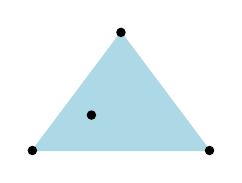
\begin{tikzpicture}[scale=1.5]
\coordinate (a) at (0,0);
\coordinate (b) at (1.5,0);
\coordinate (c) at (.75,1);

\coordinate (d) at (0.5,.3);
% \draw[green] (a) -- (d) --;
% \draw[blue] (b) -- (c);
\filldraw[LightBlue] (a) -- (b) -- (c) -- cycle;
\filldraw[black] (a) circle (1pt);
\filldraw[black] (b) circle (1pt);
\filldraw[black] (c) circle (1pt);
\filldraw[black] (d) circle (1pt);

\end{tikzpicture}
\hfill
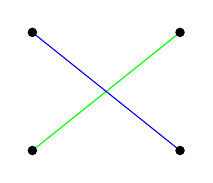
\begin{tikzpicture}[scale=1.5]
\coordinate (a) at (0,0);
\coordinate (b) at (0,1);
\coordinate (c) at (1.25,0);
\coordinate (d) at (1.25,1);
\draw[green] (a) -- (d);
\draw[blue] (b) -- (c);

\filldraw[black] (a) circle (1pt);
\filldraw[black] (b) circle (1pt);
\filldraw[black] (c) circle (1pt);
\filldraw[black] (d) circle (1pt);

% \node at (a) {\textbullet};

\end{tikzpicture}
\hfill
\caption{Four points in $\R^2$, when no three form a line. Either one is in the convex hull of the other three (left), or we may divide into pairs so that the convex hulls intersect (right).}\label{fig:Radon_example_d2}
\end{figure}
In either case, we may verify Radon's theorem.
% \missingfigure{BLue Triangle with dot in middle}
\end{remark}

\begin{proof}	
WLOG, we may take $|A|=d+2$; any surplus points we could put in $A_1,A_2$, or neither, without changing the result. Set $A=  \{v_1,v_2,\dotsc,v_{d+2}\}$. Since $v_1,v_2,\dotsc,v_{d+2}$ are affinely dependent\sidenote{since there are more than $d+1$ of them}, there exist $\alpha_1,\dotsc,\alpha_{d+2}$ with $\sum_i \alpha_i=0$ not all zero such that
\[
\alpha_1v_1 + \dotsb + \alpha_{d+2} v_{d+2} = 0.
\]
Let $A_1 = \{v_i : \alpha_i > 0\}$ and $A_2 = \{ v_i: \alpha_i < 0\}$. WLOG, $\alpha_1,\dotsc,\alpha_k > 0$ and $\alpha_{k+2},\dotsc,\alpha_{d+2} < 0$. Let $s = \alpha_1 + \dotsb + \alpha_k = - \alpha_{k+1} - \dotsb - \alpha_{d+2}$.
Then
\begin{align*}	
\left( \frac{\alpha_1}{s} \right) v_1 + \dotsb + \left( \frac{\alpha_k}{s} \right) v_{k+1} = \left( - \frac{\alpha_{k+1}}{s} \right)v_{k+1} + \dotsb + \left( - \frac{\alpha_{d+2}}{s} \right)v_{d+2}.
\end{align*}
But as shown by the LHS, this quantity lies in $\conv(A_1)$, and as shown by the RHS, the quantity lies in $\conv(A_2)$.
\end{proof}

\begin{theorem}[\cite{Caratheodory1911}]
Every point in $\conv(X)$ for $X\subset \R^d$ is a convex combination of at most $d+1$ points in $X$.
\end{theorem}
\begin{proof}	
Let $x\in \conv(X)$ be written $x = \alpha_1 v_1 + \dotsb + \alpha_n v_n$ for $v_1,\dotsc,v_n\in X$ and $\sum_i \alpha_i=0$ with $\alpha_i\geq 0$ not all zero. Suppose is $n$ is chosen minimally such that a convex combination exists. Suppose $n\geq d+2$ for the sake of contradiction. Then by Radon's theorem, wlog
\[
\conv(\{v_1,\dotsc,v_k\})\cap \conv(\{v_{k+1},\dotsc, v_n \}).
\]
So, for some $\beta_1,\dotsc,\beta_n\geq 0$,
\[
\beta_1 v_1 + \dotsb \beta_k v_k = \beta_{k+1} v_{k+1} + \dotsb + \beta_n v_n
\]
with $\sum_{i=1}^k \beta_i = \sum_{i=k+1}^n \beta_i = 1$. Then
\vspace{-\baselineskip}
\begin{fullwidth}
\begin{align}	
x &= (\alpha_1 + \epsilon \beta_1) v_1 + \dotsb + (\alpha_k + \epsilon \beta_k)v_k + (\alpha_{k+1} - \epsilon \beta_{k+1})v_{k+1}+ \dotsb +  (\alpha_n - \epsilon \beta_n)v_n \tag{$\star$} \label{eq:Cara_proof}
\end{align}
\end{fullwidth}
has the sum of coefficients one for every $\epsilon$. If $\epsilon>0$ is minimally such that $\alpha_i - \epsilon \beta_i=0$ for some $i$, then the expression \eqref{eq:Cara_proof} is a convex combination of $\{v_1,\dotsc,v_n\}\setminus \{v_i\}$, giving a contradiction.
\end{proof}
\begin{theorem}[\cite{Helly1923}]
Let $C_1,C_2\dotsc,C_n$ be a collection of convex sets in $\R^d$. If $\bigcap_{i\in I} C_i \neq \emptyset$ for every $I\subset [n]$ with $|I| = d+1$, then $\bigcap_{i=1}^n C_i \neq \emptyset$.
\end{theorem}
\begin{remark}
For $\R^1$, if we consider \marginnote{Convex sets in $\R^1$ may be open or closed intervals or rays, but we will take closed intervals for simplicity.}$C_i = [a_i,b_i]$, then if each $C_i\cap C_j\neq \emptyset$, then we need $a_i \leq b_j$ for each $i,j$. Then $[\max_i a_i, \min_i b_i] \subset C_k$ for all $k$.
\end{remark}
\begin{proof}[Proof by induction on $n$.] 
Let us postpone the base case, $n=d+2$.
For the induction step, let $C_1' = C_1 \cap C_n$, \ldots, $C_{n-1}' = C_{n-1} \cap C_n$. Then by the base case, any $(d+1)$ sets in $\{C_1',\dotsc,C_{n-1}'\}$ have a non-empty intersection. Therefore they all intersect by the induction hypothesis, hence
\[
\bigcap_{i=1}^n C_i = \bigcap_{i=1}^{n-1}C_i' \neq \emptyset.
\]
So let us show the base case. Let $v_i \in \bigcap_{j\neq i} C_j$; by the assumption. Let $A = \{v_1,\dotsc,v_{d+2}\}$. Then by Radon's theorem, there exist disjoint $A_1,A_2\subset A$ such that $\conv(A_1)\cap \conv(A_2)\neq \emptyset$. Consider $v\in \conv(A_1)\cap \conv(A_2)$. We will show that $v\in C_i$ for every $i$.

Suppose wlog that $v_i \in A_2$. Then $A_1 \subset C_i$. Since $C_i$ is convex, then $\conv(A_1) \subset C_i$. So $v\in C_i$, as desired. See \cref{fig:Helly_proof} for an example of this process in $\R^2$. \qedhere
% \missingfigure{Draw four disks in $\R^2$, $C_1,\dotsc,C_4$. Draw the $v_i$ in all the intersections but $v_i$. Connect $v_1,v_3$ in red $v_2,v_4$ in blue. Then let $v$ be the intersection. $v$ is in all four; it is in $C_1$ because it's in the interval between $v_2,v_4 \in C_1$. Etc.}
\begin{figure}
\begin{center}
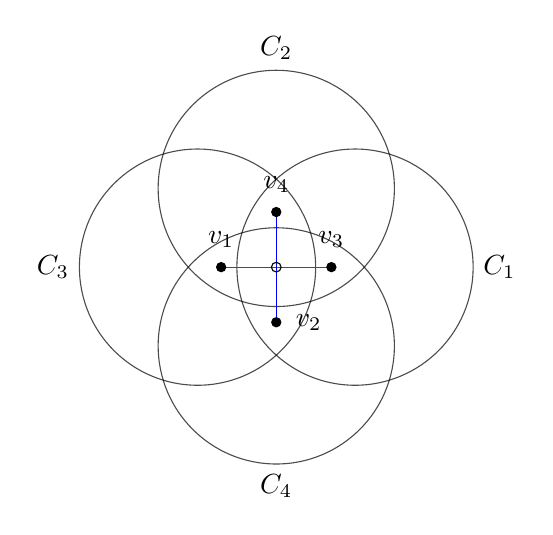
\begin{tikzpicture}[circ/.style={circle,minimum size=\circdiam cm,draw,opacity=.7}]


\def\circposrad{1}
\def\circdiam{3}

\node[circ,label={right:$C_1$}] at (0:\circposrad cm) {};
\node[circ,label={above:$C_2$}] at (90:\circposrad cm) {};
\node[circ,label={left:$C_3$}] at (180:\circposrad cm) {};
\node[circ,label={below:$C_4$}] at (270:\circposrad cm) {};

\coordinate (v3) at (0:.7cm);
\coordinate (v4) at (90:.7cm);
\coordinate (v1) at (180:.7cm);
\coordinate (v2) at (270:.7cm);

\draw[red] (-.7,0) -- (.7,0);
\draw[blue] (v2) -- (v4);

\filldraw[black] (v1) circle (1.65pt) node[label=$v_1$]{};
\filldraw[black] (v2) circle (1.65pt) node[label=right:$v_2$]{};
\filldraw[black] (v3) circle (1.65pt) node[label=$v_3$]{};
\filldraw[black] (v4) circle (1.65pt) node[label=above:$v_4$]{};

\draw (0,0) circle (1.75pt);% node[label={[label distance=.02cm]north east:$v$}]{};
\end{tikzpicture}
\end{center}
\caption{Helly's theorem in $\R^2$. Given four convex sets $C_1,\dots,C_4$ such that every triple has a non-empty intersection $v_i \in \bigcap_{j\neq i} C_j$, we can use Radon's theorem to divide $\{v_1,v_2,v_3,v_4\}$ into two disjoint sets with non-empty convex hull. Here, $A_1 = \{v_1,v_3\}$ and $A_2 = \{v_2,v_4\}$. The point in the intersection $\conv(A_1)\cap \conv(A_2)$ is labelled here with an open circle.} \label{fig:Helly_proof}
\end{figure}
\end{proof}

\begin{remark}
Helly's theorem may not apply to infinite collections of sets; consider $\{[n,+\infty):n\in \N\}$.
\end{remark}

For any set of $n$ points on the line, we can find a point such that there are at least $n/2$ points above it and below it. This is the median. How do we find an analog for $\R^d$? We'd like to find a point that in any direction away from this point, there are still many points in our set.


Let us generalize to $\R^d$: Given $X\subset \R^d$, $|X|=n$, the \defn{centerpoint} of $x$ is a point $m\in \R^d$ such that for every closed halfspace $H\subset \R^d$ such that $m\in H$, then $H$ contains at least $\frac{n}{d+1}$ points in $X$.

\begin{theorem}
For every finite set $X\subset \R^d$, there exists a centerpoint.
\end{theorem}
\begin{proof}	
Note the following are all equivalent:
\begin{itemize}
\item $m$ is a centerpoint
	\item  For every closed halfspace $H\subset \R^d$, if $m\in H$ then $|H\cap X| \geq \frac{n}{d+1}$.
	\item For every closed halfspace $H\subset \R^d$, if  $|X\cap H| < \frac{n}{d+1}$, then $m\not \in H$.
	\item For every closed halfspace $H\subset \R^d$, if $|X\cap H^c| > n - \frac{n}{d+1} = \frac{dn}{d+1}$, then $m\in H^c$.
	\item For every open halfspace $H\subset \R^d$, if $|X\cap H| >  \frac{dn}{d+1}$, then $m\in H$.
\end{itemize}
% Alternatively, every open half space which does not contain $m$ must contain at most $$
Consider the family 
\begin{align*}	
\H = \{H: H \text{ is an open halfspace of }\R^d, |H\cap X| >  \frac{dn}{d+1}\}.
\end{align*}
We will show for some $m \in \R^d$, we have $m\in H$ for every $H\in \H$, proving that $m$ is a centerpoint. 
First, if $H_1,H_2,\dotsc,H_{d+1}\in \H$, then
\begin{align*}	
H_1\cap H_2\cap \dotsm \cap H_{d+1}\neq \emptyset.
\end{align*}
Otherwise, every point of $X$ belongs to $\leq d$ out of $d+1$ of these half spaces, and thus
\begin{align*}	
dn = \sum_{i=1}^{d+1} \frac{dn}{d+1} < \sum_{i=1}^{d+1} |H_i \cap X| \leq d n
\end{align*}
which is a contradiction.

We would like to now apply Helly's theorem, but we have an infinite collection $\H$ instead of a finite one.

Let us instead set $\H' = \{ \conv(Y): Y\subset X, |Y| > \frac{dn}{d+1}\}$. By the previous argument and Helly's theorem, there exists $m\in \R^d$ such that $m\in C$ for every $C\in \H'$. But this suffices. For any $H\in \H$  there is $Y\subset X$ with $|Y| > \frac{dn}{d+1}$ and $Y\subset H$. Then $\conv(Y) \subset H$ since $H$ is convex. But since $m\in \conv(Y)$, we have $m\in H$, as desired.%if $m\not \in H$, then $m\not \in \conv(Y)$ which is a contradiction.
% If $m\not \in H$, then we want that $H$ contains
\end{proof}



\begin{theorem}[Birch]
Let $X\subset \R^2$ be a collection of $3n$ points. Then $X$ can be partitioned into $n$ triples such that the corresponding triangles all share a point in common.
\end{theorem}

\begin{figure}
\begin{center}
\begin{tikzpicture}
\begin{scope}[scale=.6]
\coordinate (v1) at (0:3cm);
\coordinate (v9) at (20:2cm);
\coordinate (v6) at (130:1cm);
\coordinate (v3) at (240:2.3cm);
\coordinate (v5) at (160:3.3cm);
\coordinate (v4) at (290:.3cm);
\coordinate (v7) at (80:1.3cm);
\coordinate (v2) at (340:1.23cm);
\coordinate (v8) at (45:3cm);
\foreach \n in {1,2,3,4,5,6,7,8,9}
{
	\filldraw (v\n) circle (1.65pt);
}
\end{scope}
\node at (3cm,0){$\leadsto$};
\begin{scope}[scale=.6, xshift=10cm]
\coordinate (v1) at (0:3cm);
\coordinate (v9) at (20:2cm);
\coordinate (v6) at (130:1cm);
\coordinate (v3) at (240:2.3cm);
\coordinate (v5) at (160:3.3cm);
\coordinate (v4) at (290:.3cm);
\coordinate (v7) at (80:1.3cm);
\coordinate (v2) at (340:1.23cm);
\coordinate (v8) at (45:3cm);
\foreach \n in {1,2,3,4,5,6,7,8,9}
{
	\filldraw (v\n) circle (1.65pt);
}

\filldraw[blue,opacity=.4] (v7) -- (v4) -- (v1) -- cycle;

\filldraw[green,opacity=.4] (v2) -- (v5) -- (v8) -- cycle;

\filldraw[red,opacity=.4] (v3) -- (v6) -- (v9) -- cycle;
\end{scope}


\end{tikzpicture}
\end{center}
\caption{An example of Birch's theorem with nine points. On the left, the nine points are depicted; on the right, intersecting triangles chosen.}\label{fig:birch_ex}
\end{figure}
% \missingfigure{Draw 9 points and three triangles in different colors so that there is a common area. Label a point of intersection.}
\begin{remark}
See \cref{fig:birch_ex} for an example.
\end{remark}\begin{proof}
% \missingfigure{Draw rays from centerpoint to each vertex}

Let $m$ be a centerpoint of $X$. Label the points of $X$ by $x_1$, $x_2$, \ldots, $x_{3n}$ so that the rays $mx_1$, $mx_2$, \ldots, $mx_{3n}$ are arranged around $m$ in clockwise order, as shown in \cref{fig:birch_proof1}.
\begin{figure}[ht]
\begin{center}
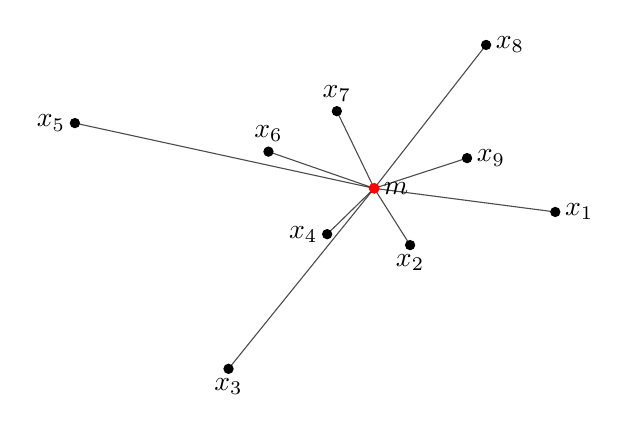
\begin{tikzpicture}
\begin{scope}[scale=1]
\coordinate (m) at (.7cm,.3cm);
\coordinate (v1) at (0:3cm);
\coordinate (v9) at (20:2cm);
\coordinate (v6) at (130:1cm);
\coordinate (v3) at (240:2.3cm);
\coordinate (v5) at (160:3.3cm);
\coordinate (v4) at (290:.3cm);
\coordinate (v7) at (80:1.3cm);
\coordinate (v2) at (340:1.23cm);
\coordinate (v8) at (45:3cm);
\foreach \n in {6,7}
{
	\filldraw (v\n) circle (1.65pt) node[above]{$x_\n$};
}
\foreach \n in {4,5}
{
	\filldraw (v\n) circle (1.65pt) node[left]{$x_\n$};
}
\foreach \n in {1,8,9}
{
	\filldraw (v\n) circle (1.65pt) node[right]{$x_\n$};
}
\foreach \n in {2,3}
{
	\filldraw (v\n) circle (1.65pt) node[below]{$x_\n$};
}

% \filldraw[blue,opacity=.4] (v5) -- (v4) -- (v1) -- cycle;

% \filldraw[green,opacity=.4] (v3) -- (v9) -- (v8) -- cycle;

% \filldraw[red,opacity=.4] (v6) -- (v7) -- (v2) -- cycle;

	\foreach \n in {1,2,...,9}
{
	\draw[opacity=.7] (m) -- (v\n);
}
	\filldraw[red] (m) circle (1.75pt) node[black,right]{$m$};

\end{scope}
\end{tikzpicture}
\end{center}
\caption{Nine points $\{x_1,\dotsc,x_9\}$ in $\R^2$ and their centerpoint $m$, in red. Continuing the example from \cref{fig:birch_ex}, the points are labelled clockwise in order from the centerpoint. }\label{fig:birch_proof1}
\end{figure}
Let $X_i = \{ x_i, x_{i+n}, x_{i+2n}\}$ for $i=1,\dotsc, n$. Then $m\in \conv(X_i)$ for each $i$.

Assume $m\not \in \conv(X_i)$. Then\sidenote{We are appealing to a separating hyperplane theorem, such as \cite[Theorem 1.24]{matouvsek2002lectures}, although the result seems clear geometrically in this case.} some closed halfplane containing $m$ separates $m$ from the three points of $X_i$; see \cref{fig:birch_proof2}. But then the $2n$ rays between $x_i$ and $x_{i+2n}$ fall in the other half of the halfplane, so there are at least $2n+1$ points in $X$ on the other side, contradicting that $m$ is a centerpoint. \qedhere
\begin{marginfigure}
\begin{center}
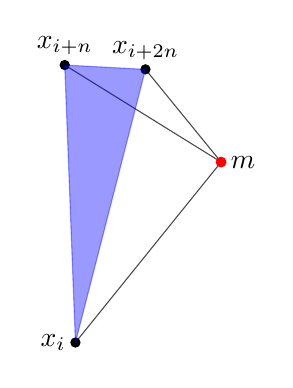
\begin{tikzpicture}
\coordinate (v3) at (240:2.3cm);
\coordinate (v2) at (100:1.5cm);
\coordinate (v1) at (130:2cm);
\coordinate (m) at (.7cm,.3cm);
\foreach \n in {1,2,3}
{
	\draw[opacity=.7] (m) -- (v\n);
}
	\filldraw (v3) circle (1.65pt) node[left]{$x_i$};
	\filldraw (v2) circle (1.65pt) node[above]{$x_{i+2n}$};
	\filldraw (v1) circle (1.65pt) node[above]{$x_{i+n}$};


\filldraw[blue,opacity=.4] (v1) -- (v2) -- (v3) -- cycle;
	\filldraw[red] (m) circle (1.75pt) node[black,right]{$m$};

\end{tikzpicture}

\end{center}
\caption{The case where the centerpoint $m$, in red, is not in the convex hull of $X_i$, shown in blue. Then the $2n$ points $\{x_i,x_{i+1},\dotsc,x_{i+2n}$ all lie between $x_i$ and $x_{i+2n}$ (angularly) and may be separated from $m$ by a closed hyperplane, contradicting the definition of centerpoint.} \label{fig:birch_proof2}
\end{marginfigure}
% \missingfigure{$m$, then line, and three points $x_i$, $x_{i+n}$, $x_{i+2n}$. Draw outline convex hull in red  around those three. They are all on the other side of a halfplane from $m$.}

\end{proof}

\begin{theorem}[Colorful Carath\'eodory theorem, \cite{barany1982generalization}]
Let $S_1,S_2,\dotsc,S_{d+1}\subset \R^d$ and suppose that $x\in \bigcap_{i=1}^{d+1} \conv(S_i)$. Then there exist $x_1\in S_1$, $x_2\in S_2$, \ldots, $x_{d+1}\in S_{d+1}$ such that $x\in \conv(\{x_1,x_2,\dotsc,x_{d+1}\})$.
\end{theorem}
\begin{remark}
The different sets correspond to different colors. Then $x$ belongs to a convex combination of points each a different color. Taking each set $S_i \equiv X$, we recover Carath\'eodory's theorem.
\end{remark}
\begin{proof}	
We will say $C$ is a \defn{colorful simplex} if $C = \conv(\{ x_1,x_2,\dotsc,x_{d+1} \})$ for $x_i\in S_i$ for $i\in[d+1]$. Suppose that no colorful simplex contains $x$.

Choose a colorful simplex $C$ such that $\dist(C,x) = \min_{c\in C} \|c-x\|$ is minimal.\marginnote{$\|c-x\| = \dist(c,x)$ is the 2-norm (Euclidean norm).}

Let $z\in C$ be the closest point to $x$: $\dist(z,x) = \dist(C,x)$.


Let $H$ be a hyperplane orthogonal to $zx$ through $z$. Let $H^+$ and $H^-$ be closed halfspaces with respect to $H$ such that $x\in H^-$.

\begin{claim}
$C\subset H^+$.
\end{claim}
\begin{subproof}	
Suppose not: $z' \in C\cap (H^- \setminus H^+)$\marginnote{So $z'\not \in H^+$}. Then angle $z' z x$ is acute and points on $zz'$ near $z$ are closer to $x$ than $z$, a contradiction.
\end{subproof}

\begin{claim}
$z\in \conv(\{x_1,\dotsc,x_{d+1}\}\cap H)$.
\end{claim}
\begin{subproof}	
$z = \sum_{i=1}^{d+1} \lambda_i x_i$ with $\lambda_i\geq 0$, $\sum_i \lambda_i =1$, since $z\in C$. Let $f: \R^d \to \R$ linear such that if $f(p)> 0$ for $p\in H^+\setminus H$, and $f(p) = 0$ for $p\in H$. 

Then $0 = f(z) = \sum_{x_i \in H^+ \setminus H} \lambda_i \underbrace{f(x_i)}_{>0} + \sum_{x_i \in H} \lambda_i \underbrace{f(x_i)}_{=0}$. So we must have $\lambda_i=0$ when $x_i \in H^+ \setminus H$.
\end{subproof}

By Caratheordy theorem applied to $z$ and $\{x_i,\dotsc,x_{d+1}\}\cap H$, there exists $j$ such that \begin{align*}	
z\in \conv((\{x_1,x_2,\dotsc,x_{d+1}\}\setminus \{j\})\cap H).
\end{align*}
We know $x\in \conv(S_j)$, so there exists $x'_j \in S_j \cap (H^-\setminus H^+)$. Let $C' = \conv( \{x_1,\dotsc,x_{j-1},x_j',x_{j+1},\dotsc,x_{d+1}\})$.

\begin{claim}
Then $\dist(C',x) < \dist(C,x)$.
\end{claim}
\begin{subproof}	
We know $z\in C'$. Then, as before, points on $x_j' z\subset C'$ are closer to $x$ than $z$. 
\end{subproof}
This last claim yields a contradiction to minimality of $C$.

Note: we assumed the $S_i$ were finite when assuming there exists a minimal colorful simplex $C$. But in fact, we only need to consider $\conv(S_i)$, which only depends on $d+1$ points, by (the original) Carath\'eodory points. Thus, we could take $|S_i|=d+1$ for each $i$.
\end{proof}
\begin{remark}
This proof yields an algorithm to improve our convex set one point at a time to the optimal one. Yet, it is unknown if this algorithm or any other can find the optimal $\conv(\{x_1,\dotsc,x_{d+1}\})$ in polynomial time.
\end{remark}

\begin{theorem}[\cite{Tverberg1966}]
Let $A\subset \R^d$ with $|A| \geq (r-1)(d+1)+1$. Then there exist $A_1,A_2,\dotsc,A_r\subset A$ pairwise disjoint such that $\bigcap_{i=1}^r \conv(A_i)\neq \emptyset$.
\end{theorem}
\begin{remark}
Radon's theorem is the case $r=2$. If $d=1$, then we have $2r-1$ points in $\R$ which we wish to write as $r$ groups with intersecting convex hulls.

For $d=2$, $3r-2$ points in $\R^2$ can be partitioned into $r$ groups with intersecting convex hulls. This in fact implies Birch's theorem.
\end{remark}

If $u\in \R^n$ and $v\in \R^m$, then $u\otimes v \in \R^{nm}$. Suppose $u = (u_1,\dotsc,u_n)$ and $v = (v_1,\dotsc,v_m)$; i.e., we have chosen bases for $\R^n$ and $\R^m$. Then $u\otimes v $ can be thought of as a $m\times n$ matrix with components $(u\otimes v)_{ij} = u_i v_j$.
\begin{align*}	
u = \begin{pmatrix}
u_1\\ u_2\\ u_3
\end{pmatrix}, \qquad v = \begin{pmatrix}
v_1 \\ v_2 \\ v_3
\end{pmatrix}, \qquad u\otimes v = \begin{pmatrix}
u_1 v_1 & u_1 v_2 & u_1 v_3\\
u_2 v_1 & u_2 v_2 & u_2 v_3 \\
u_3 v_1 & u_3 v_2 & u_3 v_3
\end{pmatrix}.
\end{align*}

\begin{proposition}
~\begin{enumerate}
\item $(\alpha_1 u_1 + \alpha_2 u_2) \otimes v = \alpha_1 (u_1\otimes v) + \alpha_2 (u_2\otimes v)$
\item  Suppose $v_1,\dotsc,v_k$ are linearly independent and $u_1\otimes v_1 + u_2\otimes v_2 + \dotsm + u_k \otimes v_k = 0$. Then $u_1 = u_2 = \dotsm = u_k = 0$.
\end{enumerate}
\end{proposition}
We will leave the proof of the proposition as an exercise, and proceed to the proof of Tverberg's theorem.
\lect{3}{23}
% \marginnote{Lecture X: March 23, 2016.}

\begin{proof}[Proof (\cite{sarkaria1992tverberg}).]
Let $m = (r-1)(d+1)+1$.

\begin{enumerate}
	\item Instead of the orginal setting, consider $A = \{v_1,v_2,\dotsc,v_m\} \subset \R^{d+1}$ such that the vectors of $A$ lie in an affine hyperplane not passing through the origin. I.e., there exists $f: \R^{d+1}\to \R$ linear such that $f(v_i) = 1$ for every $i$. 
	\item Let $w_1,w_2,\dotsc,w_r$ be vectors in $\R^{r-1}$ such that $w_1+w_2+\dotsc+w_r=0$ and this is essentially the only relation between these vectors. For instance, we could choose $w_i = (\underbrace{0,\dotsc,0}_{i-1},1,0,\dotsc,0)$ for $i=1,\dotsc,r-1$ and $w_r = (-1,-1,\dotsc,-1)$.
	\item Consider $\{v_i \otimes w_j: 1\leq i \leq m, 1\leq j \leq r\}\subset \R^{d+1}\otimes \R^{r-1}\cong \R^{m-1}$. For each $i$, we may think of $S_i:=\{v_i\otimes w_j:1\leq j\leq r\}$ as a copy of the $w_j$ embedded in a hyperplane. Note $0\in \conv(S_i)$ for each $i$, since
	\begin{align*}	
	0 &= \frac{1}{r}v_i \otimes (w_1+w_2+\dotsm+ w_r) = \frac{1}{r} v_i \otimes w_1 + \frac{1}{r}v_i\otimes w_2  +\dotsm + \frac{1}{r}v_i\otimes w_r.
	\end{align*}
	\item Apply the Colorful Carath\'eodory theorem to $S_1,\dotsc,S_m$ and the point $0$. We get that for $1\leq i\leq m$ there exist $j_i$ and $\lambda_i\geq 0$ such that
	\begin{align}	
	\sum_{i=1}^m \lambda_i (v_i\otimes w_{j_i})=0 \label{eq:Tv_conv_comb}
	\end{align}
	with $\sum_i \lambda_i=1$.

	Let $A_j = \{ v_i : j_i = j \}$ for $j=1,\dotsc,r$. Let us rewrite \cref{eq:Tv_conv_comb} as follows.
	\begin{align*}	
	\sum_{j=1}^r \left( \sum_{v_i \in A_j} \lambda_i v_i \right)\otimes w_j = 0.
	\end{align*}
	Let us write $u_j =  \sum_{v_i \in A_j} \lambda_i v_i$. Then we have
	\begin{align*}	
	u_1\otimes w_1 + u_2\otimes w_2 + \dotsm + u_r\otimes w_r &= 0\\
	(u_1- u_r)\otimes w_1 + (u_2-u_r)\otimes w_2 + \dotsm + (u_{r-1} - u_r)\otimes w_{r-1} &= 0
	\end{align*}
	using $w_r = -w_1 - w_2 - \dotsm - w_{r-1}$. But since $\{w_1,\dotsc,w_{r-1}\}$ are linearly independent, we must have $u_1-u_r = u_2 - u_r = \dotsm = u_{r-1}- u_r = 0$. That is, 
	\[
	u_1 = u_2 = \dotsm = u_r.
	\]
	Substituting the definition of $u_j$,
	\begin{align}	
	\sum_{v_i \in A_1} \lambda_i v_i = \sum_{v_i\in A_2} \lambda_i v_i = \dotsm = \sum_{v_i\in A_r}\lambda_i v_i. \label{eq:Tv_lambda_vs_equal}
	\end{align}
	Suppose the sum of coefficients $\lambda_i$ in each expression is the same and is equal to $s$.\marginnote{In fact, $s= \frac{1}{r}$.} Then
	\begin{align*}	
	\sum_{v_i \in A_1} \frac{\lambda_i}{s}v_i = \dotsm = \sum_{v_i\in A_r} \frac{\lambda_i}{s}v_i = p
	\end{align*}
	and hence $p\in \conv(A_k)$.

	But if we apply $f$ to \cref{eq:Tv_lambda_vs_equal}, by linearity we obtain
	\begin{align*}	
	\sum_{v_i \in A_1} \lambda_i f(v_i) = \sum_{v_i\in A_2} \lambda_i f(v_i) = \dotsm = \sum_{v_i\in A_r}\lambda_i f(v_i). 
	\end{align*}
	Since $f(v_i)=1$ for all $i$, we find $\sum_{v_i\in A_j} \lambda_i \equiv s$. \qedhere
\end{enumerate}
\end{proof}
\flavor{A magical proof. 30 years after the original.}

\begin{remark}
In Helly's theorem, we consider $C_1,\dotsc,C_n\subset \R^d$ convex such that every $(d+1)$-tuple of $C$'s has non-empty intersection. Then we obtain that there is a common point in all of the sets. Suppose instead $\sim \frac{1}{2}$ of the $(d+1)$-tuples have a non-empty intersection. What can we say about large intersections?
\end{remark}
\begin{theorem}[Fractional Helly's theorem]
For every $d\in \N$ and $0< \alpha \leq 1$ there exists a $\beta = \beta(\alpha,d)$ such that the following holds. Let $C_1, C_2,\dotsc,C_n\subset \R^d$ be convex and suppose $\bigcap_{i\in I} C_i\neq \emptyset$ for at least $\alpha {n\choose d+1}$ sets $I\subset[n]$ with $|I| = d+1$. Then there exists $X \subset [n]$ with $|X|\geq \beta n$ such that $\bigcap_{i\in X} C_i \neq \emptyset$.

\end{theorem}
\begin{proof}	
We need to assume that $C_1,C_2,\dotsc,C_n$ are compact; we may do this as follows. For each set $I$ as in the statment, select $p_I \in \bigcap_{i\in I} C_i$. Then replace $C_i$ by $\conv(\{p_I:  I \text{ s.t. } I\ni i\})$.

Let $F_I = \bigcap_{i\in I} C_i$. Let $<$ be a linear lexicographic order on $\R^d$. Let $p_I= \min (F_I)$ in this order, if $F_I\neq \emptyset$. Since $F_I$ is compact, $p_I$ exists and is unique.

\begin{claim}
For every $I\subset[n]$ with $|I|=d+1$, s.t. $F_I\neq \emptyset$, there exists $J\subset I$, $|J| = d$ such that $p_I = p_J$.
\end{claim}
\begin{remark}
For any $J\subset I$,  we have $p_J \leq P_I$.
\end{remark}
\begin{subproof}[Proof of claim.]
Let $C =  \{q \in \R^d: q< p_I\}$. Then $C$ is convex. Then $C\cap \left( \bigcap_{i\in I} C_i \right) = C\cap F_I = \emptyset$. Since this $(d+2)$-tuple intersection is empty, then by the contrapositive of Helly's theorem, not all $(d+1)$-tuples can have empty intersection. But since $F_I\neq \emptyset$, the $(d+1)$-tuple with empty intersection must include $C$. So there exists $J\subset I$ with $|J| = d$ such that
\begin{align*}	
C \cap \left( \bigcap_{i\in J}C_i \right) = \emptyset.
\end{align*}
Then $p\geq p_I$ for every $p\in F_J$.
\end{subproof}

Now for every $I\subset[n]$ with $|I| = d+1$, $F_I\neq \emptyset$, select $J\subset I$ with $|J| = d$ such that $P_J = P_I$. Then there are $\alpha{n \choose d+1}$ sets $I$ which we consider, and  ${n\choose d}$ sets $J$ of size $d$. So some set $J_0$ is associated with at least $\frac{\alpha {n\choose d+1}}{{n\choose d}}$ sets $I$. Such sets are of the form $J_0 \cup \{ i\}$ for some $i$, and $p_{J_0} \in C_i$ for such $i$. So $p_{J_0}$ belongs to  at least 
\begin{align*}	
\frac{\alpha{ n\choose d+1}}{{n\choose d}} + d = \frac{\alpha(n-d)}{d+1}+d \geq \frac{\alpha}{d+1}n
\end{align*}
sets $C_i$ (counting the $d$ sets in $J_0$).
Therefore, we may take $\beta = \frac{\alpha}{d+1}$.
\end{proof}
\begin{remark}
This constant is not optimal; for instance, when $\alpha=1$, we would like $\beta=1$ to recover Helly's theorem. The optimal constant is known, however.
\end{remark}


For every $k$, we'd like to prove existence (and estimate the value) of the number $g(k)$ such that in every set of $g(k)$ points in $\R^2$, with no three lying on a line\sidenote[][-1cm]{``in general position''} there exist $k$ points which are convexly independent\sidenote[][-1cm]{``in convex position,'' or are the verticies of a convex polygon}.

Let us consider small $k$. Then $g(1)=1$, $g(2)=2$, $g(3)=3$. But $g(4) > 4$, as shown in \cref{fig:g4}.
\begin{marginfigure}[-1cm]
\begin{center}
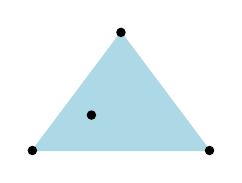
\begin{tikzpicture}[scale=1.5]
\coordinate (a) at (0,0);
\coordinate (b) at (1.5,0);
\coordinate (c) at (.75,1);

\coordinate (d) at (0.5,.3);
% \draw[green] (a) -- (d) --;
% \draw[blue] (b) -- (c);
\filldraw[LightBlue] (a) -- (b) -- (c) -- cycle;
\filldraw[black] (a) circle (1pt);
\filldraw[black] (b) circle (1pt);
\filldraw[black] (c) circle (1pt);
\filldraw[black] (d) circle (1pt);

\end{tikzpicture}
\end{center}
\caption{An illustration of the fact that $g(4) > 4$. We have four points with no three lying on a line such that not all four are convexly independent: one point is in the convex hull of the other three.} \label{fig:g4}
\end{marginfigure}

\begin{lemma} \label{lem:g4_is_5}
$g(4)=5$.
\end{lemma}
\begin{proof}	
Let $X\subset \R^2$ be a set of five points in general position. Consider $\conv(X)$: this is a polygon with 3, 4, or 5 vertices. If there are 4 or 5 vertices we are done, so, assume $\conv(X)$ is a triangle with vertices $\{a,b,c\}$. Let $\{d,e\}$ be the remaining two points of $X$, as shown in \cref{fig:lem89convX}.
\begin{figure}
\begin{center}
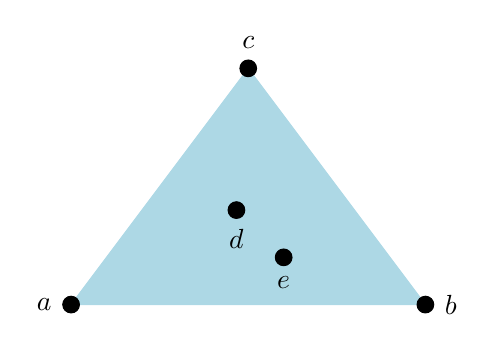
\begin{tikzpicture}[scale=3]
\coordinate (a) at (0,0);
\coordinate (b) at (1.5,0);
\coordinate (c) at (.75,1);

\coordinate (e) at (0.9,.2);
\coordinate (d) at (0.7,.4);

% \draw[green] (a) -- (d) --;
% \draw[blue] (b) -- (c);
\filldraw[LightBlue] (a) -- (b) -- (c) -- cycle;
	\filldraw[black] (a) circle (1pt) node[label=left:$a$]{};
\filldraw[black] (b) circle (1pt)node[label=right:$b$]{};
\filldraw[black] (c) circle (1pt)node[label=above:$c$]{};
\filldraw[black] (d) circle (1pt)node[label=below:$d$]{};
\filldraw[black] (e) circle (1pt)node[label=below:$e$]{};

\end{tikzpicture}
\end{center}
\caption{We assume $\conv(X) = \conv(\{a,b,c\})$; then $\{d,e\}:= X\setminus \{a,b,c\}$ lie inside the triangle formed by $\{a,b,c\}$.} \label{fig:lem89convX}
\end{figure}

Now assume the line $de$ intersects $ab$ and $ac$, as shown in \cref{fig:lem89de_line}.
\begin{marginfigure}
\begin{center}
\usetkzobj{all}
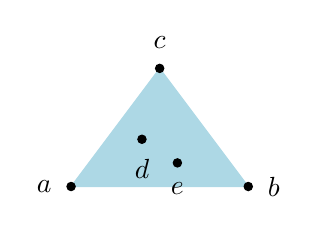
\begin{tikzpicture}[scale=1.5]
\coordinate (a) at (0,0);
\coordinate (b) at (1.5,0);
\coordinate (c) at (.75,1);

\coordinate (e) at (0.9,.2);
\coordinate (d) at (0.6,.4);

% \draw[green] (a) -- (d) --;
% \draw[blue] (b) -- (c);
\filldraw[LightBlue] (a) -- (b) -- (c) -- cycle;
	\filldraw[black] (a) circle (1pt) node[label=left:$a$]{};
\filldraw[black] (b) circle (1pt)node[label=right:$b$]{};
\filldraw[black] (c) circle (1pt)node[label=above:$c$]{};
\filldraw[black] (d) circle (1pt)node[label=below:$d$]{};
\filldraw[black] (e) circle (1pt)node[label=below:$e$]{};



  % \tkzDefLine[through d](d,e)
  \tkzDrawLine[add = 2 and 2](d,e)
\end{tikzpicture}
\end{center}
\caption{We assume the line passing through $d$ and $e$ intersects the sides $ac$ and $ab$ of the triangle. Since no three points in $X$ are colinear, the line passing through $d$ and $e$ must intersect two of the sides of the triangle, so we can always relabel the verticies so that this is the case.} \label{fig:lem89de_line}
\end{marginfigure} Then $bcde$ form a convex quadrangle. We may see this by taking the convex hull of any three of $\{b,c,d,e\}$ to form a triangle $T$, and calling the omitted point $z$. Then there are two boundary line segments of the quadrilateral $bcde$ which end in $z$, but each of these line segments only intersects $T$ at the opposite end from $z$. If $z\in T$, then the whole line between $z$ and those endpoints would have to be included in $T$. Thus, $z\not \in T$, and we truly have a convex quadrilateteral $bcde$. This is illustrated in \cref{fig:lem89T}.
\begin{figure}
\begin{center}
\begin{tikzpicture}[scale=3]
\coordinate (a) at (0,0);
\coordinate (b) at (1.5,0);
\coordinate (c) at (.75,1);

\coordinate (e) at (0.9,.2);
\coordinate (d) at (0.7,.4);

% \draw[green] (a) -- (d) --;
% \draw[blue] (b) -- (c);
\filldraw[LightBlue] (a) -- (b) -- (c) -- cycle;
	\filldraw[black] (a) circle (1pt) node[label=left:$a$]{};
\filldraw[black] (b) circle (1pt)node[label=right:$b$]{};
\filldraw[black] (c) circle (1pt)node[label=above:$c$]{};
\filldraw[black] (d) circle (1pt)node[label=below:$d$]{};
\filldraw[black] (e) circle (1pt)node[label=below:$e$]{};

\filldraw[pattern=north west lines] (c) -- (d) -- (b) -- cycle;

\draw[dashed] (d)--(e);
\draw[dashed] (e)--(b);

\end{tikzpicture}
\end{center}
\caption{We will take $T= \conv(\{c,d,b\})$, the crosshatched region. Then the two dashed lines only intersect $T$ at the verticies $d,b$. We see if $e$ were moved up into $T$, then the line passing through $d$ and $e$ would no longer intersect the segment $ab$.} \label{fig:lem89T}
\end{figure}
\end{proof}
\begin{theorem}[\cite{erdosszekeres1935combinatorial}]
$g(k)$ exists for all $k$.
\end{theorem}
\begin{proof}	
Let $n=g(k)$ be such that in every coloring of $[n]^{(4)}$ in colors red and blue, one can find either a set of $5$ with all quadruples in red, or a set of size $k$ with all quadruples blue. This exists by the Hypergraph Ramsey theorem\sidenote{For all positive integers $r,k_1$, and $k_2$ there exists a positive integer $n= R^{(r)}(k_1,k_2)$ so that the following holds. If elements of $[n]^{(r)}$ are colored in colors red and blue then there is a set $Z\subset [n]$ such that either $|Z| = k_1$ and all elements of $Z^{(r)}$ are red, or $|Z| = k_2$ and all elements of $Z^{(r)}$ are blue.}.

Color quadruples of points in red color if it is not in convex position, and otherwise in blue. By  \cref{lem:g4_is_5}, there exists a set of $k$ points such that every four of them are in convex position.

Then these $k$ points are in convex position by Carath\'eodory's theorem.
\end{proof}
\begin{remark}
We may obtain much better bounds by longer proofs.
\end{remark}

